\documentclass[12pt]{article}
\usepackage{amsmath,amsfonts}
\usepackage{enumerate}
\usepackage{graphicx}
\usepackage{float}
\usepackage{multirow}
\usepackage{booktabs}
\usepackage{placeins}

\renewcommand{\baselinestretch}{1}
\topmargin 0in \headheight 0.0in \textheight 9in \textwidth 6.5in
\oddsidemargin 0.1in \evensidemargin 0.1in

\graphicspath{{/Users/siyangren/Documents/ra-cida/ESFGSP_Paper/Simulations/results/figures}}


\begin{document}


\section*{Methods}

We evaluate the performance of LASSO models in identifying significant features in high-dimensional datasets, comparing model performance in the pixel space and the frequency space. Two simulations were designed: one simulating data in the pixel space and the other in the frequency space. After each simulation, the generated data is projected between spaces, and LASSO models are fitted in both spaces to assess performance.

\subsection*{Transformation Between Pixel and Frequency Spaces}

Let \( \mathbf{x} \) be a column vector of pixel values for an image with 256 pixels. The pixel values exhibit inherent correlations, captured by the covariance matrix \( \Sigma \). Performing eigen-decomposition of \( \Sigma \), we obtain a matrix \( V \), where each column is an eigenvector of \( \Sigma \). Using \( V \), the transformation from the pixel space to the frequency space is expressed as:

\[
\mathbf{x}_{\text{freq}} = V^T \mathbf{x}
\]

In the frequency space, the covariance matrix of \( \mathbf{x}_{\text{freq}} \) is \( V^T \Sigma V \), which is diagonal. This diagonal structure implies that the features in the frequency space are uncorrelated. We can simulate \( \mathbf{x} \) for 1000 times, with each iteration as a row and use \( \mathbf{X} \) to represent it.

\subsection*{Simulation Design}

Two simulations were conducted, generating 1000 observations, each with 256 features representing \( 16 \times 16 \) pixel images. Both simulations were repeated over 500 iterations to ensure robustness.

\subsubsection*{Simulation 1: Data Generated in the Pixel Space}

In the first simulation, data is generated in the pixel space. The covariates \( \mathbf{X} \) follow an exponential correlation structure, where the covariance between pixels \( i \) and \( j \) is given by:

\[
\Sigma_{i j} = \exp(-\text{dist}(i, j))
\]
where \( \text{dist}(i, j) \) is the distance between pixels in the 2D space. The coefficient vector \( \beta \) is sparse, with non-zero values confined to a central \( 8 \times 8 \) region of the image. The response variable \( y \) is drawn from a binomial distribution, with the probability \( p \) determined by:

\[
\eta = \mathbf{X} \beta, \quad p = \frac{1}{1 + \exp(-\eta)}
\]

The non-zero coefficients in \( \beta \) are chosen to ensure that \( p \) is uniformly distributed within \( [0, 1] \).

Once the data is generated in the pixel space, we project it to the frequency space using the transformation \( \mathbf{X}_{\text{freq}} = \mathbf{X} V \), and calculate the corresponding coefficients \( b = V^T \beta \).

\subsubsection*{Simulation 2: Data Generated in the Frequency Space}

In the second simulation, data is generated directly in the frequency space. The covariance matrix in this space is diagonal, representing no correlation between features. We assume a diagonal covariance matrix with decreasing diagonal values, corresponding to decreasing variance across frequencies.

The coefficient vector \( b \) is sparse, with 10\% of the 256 entries randomly assigned non-zero values, while the remaining entries are set to zero. The response variable \( y \) is generated similarly to the first simulation, ensuring that \( p \) is uniformly distributed.

Once the data is generated in the frequency space, we project it back to the pixel space using the inverse transformation \( \mathbf{X} = \mathbf{X}_{\text{freq}} V^T \), and calculate the corresponding coefficients \( \beta = V b \).

\subsection*{Model Fitting and Evaluation}

For both simulations, we fit LASSO models using the covariates in both the pixel space and the frequency space. Each dataset, consisting of 1000 observations with 256 features, is split into training (80\%) and test (20\%) sets. The regularization parameter \( \lambda \) is tuned using cross-validation based on binomial deviance. Two specific values of \( \lambda \) are considered:

\begin{itemize}
    \item \( \lambda_{\text{min}} \): The value of \( \lambda \) that minimizes the cross-validated error.
    \item \( \lambda_{\text{1se}} \): The largest value of \( \lambda \) within one standard error of the minimum.
\end{itemize}

After selecting the optimal \( \lambda \), model performance is evaluated using accuracy and the Area Under the Curve (AUC) metric. Additionally, a permutation test is performed 100 times to calculate p-values for each covariate. Across all iterations, we compute the mean and standard deviation of the performance metrics and the percentage of significant p-values for each covariate.


\section*{Results}

\subsection*{Effect Size Determination}

In Simulation 1, the distribution of the success probability \( p \) was evaluated at various \( \beta \) values: 0.01,
0.05, 0.1, 0.2, and 1. As shown in Figure \ref{fig:sim1_p_dist}, \( \beta = 0.1 \) yielded the most uniform distribution
of \( p \), making it the optimal choice for model fitting. Similarly, in Simulation 2, the distribution of \( p \) was assessed at various \( b \) values: 0.1, 0.2, 0.4, 0.6, 0.8, and 1. As illustrated in Figure \ref{fig:sim2_p_dist}, \( b = 0.2 \) resulted in the most uniform distribution of \( p \). 

\begin{figure}[h!] 
	\centering
	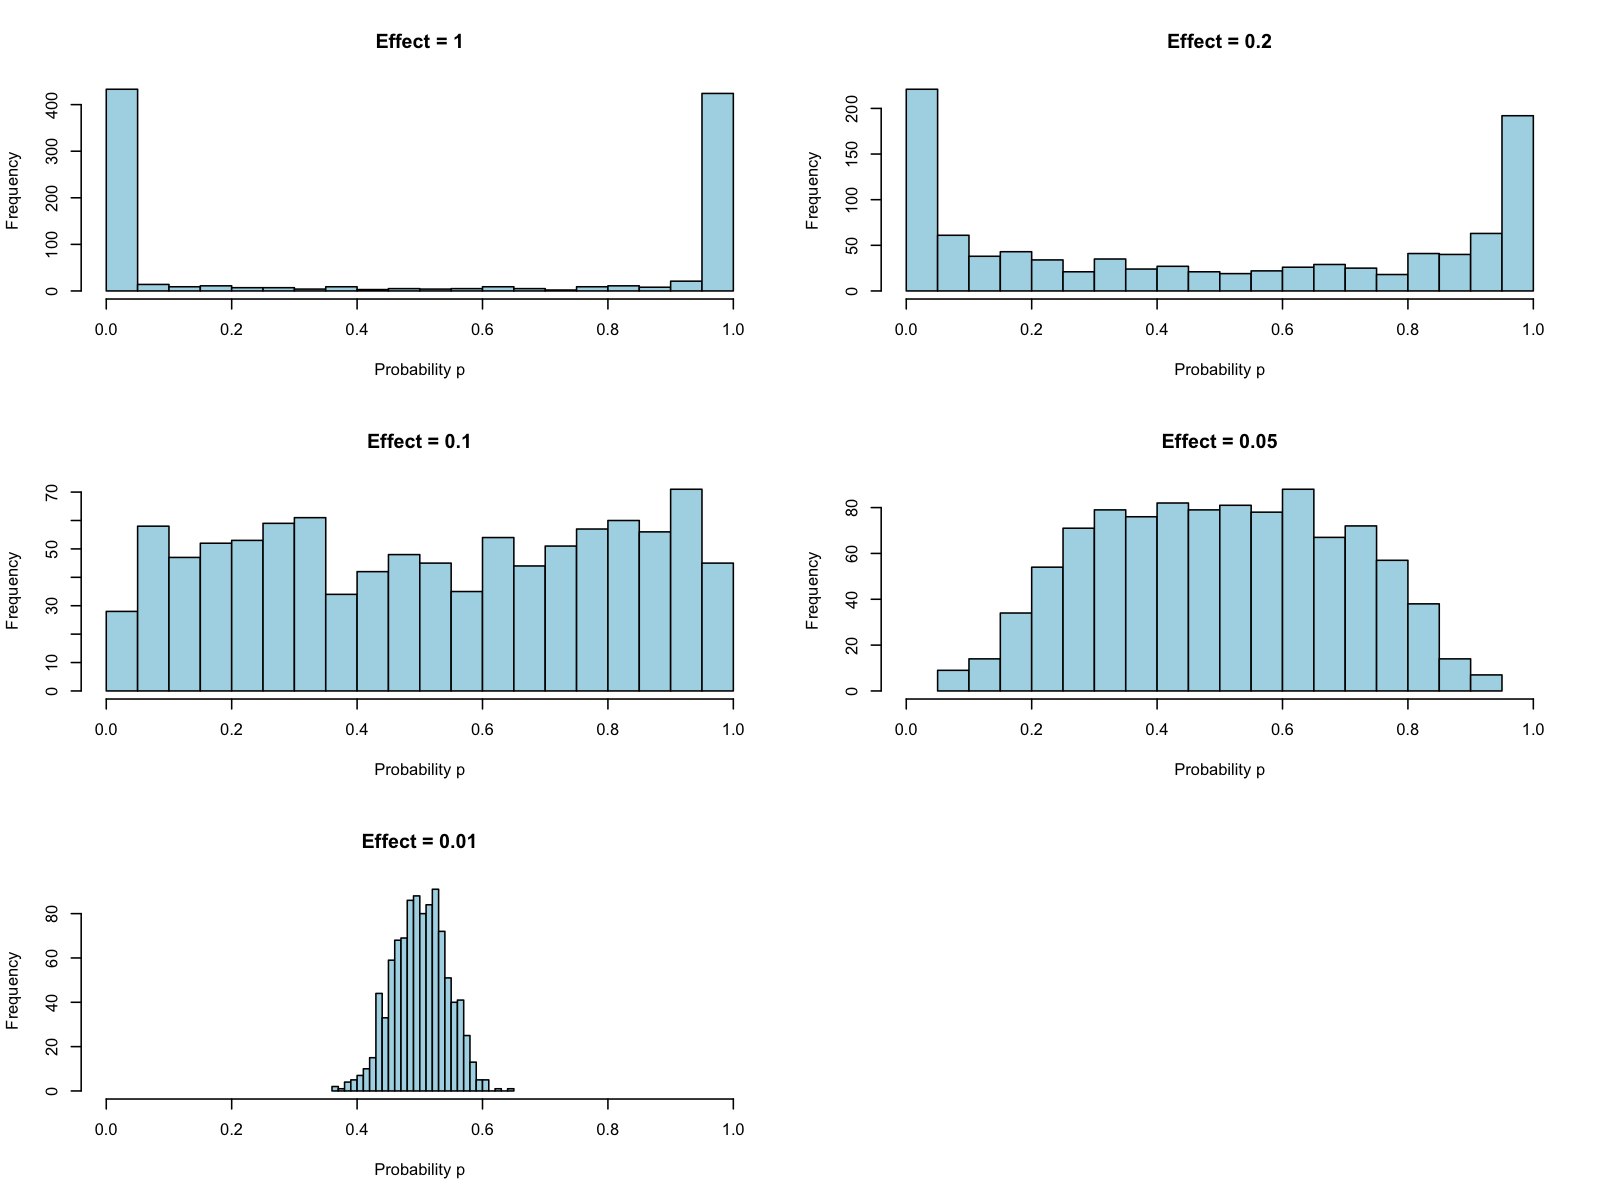
\includegraphics[width=0.8\textwidth]{sim1_p_dist.png} 
  \caption{Distribution of success probability \( p \) at different \( \beta \) values in Simulation 1.}
	\label{fig:sim1_p_dist} 
\end{figure}

\begin{figure}[h!] 
	\centering
	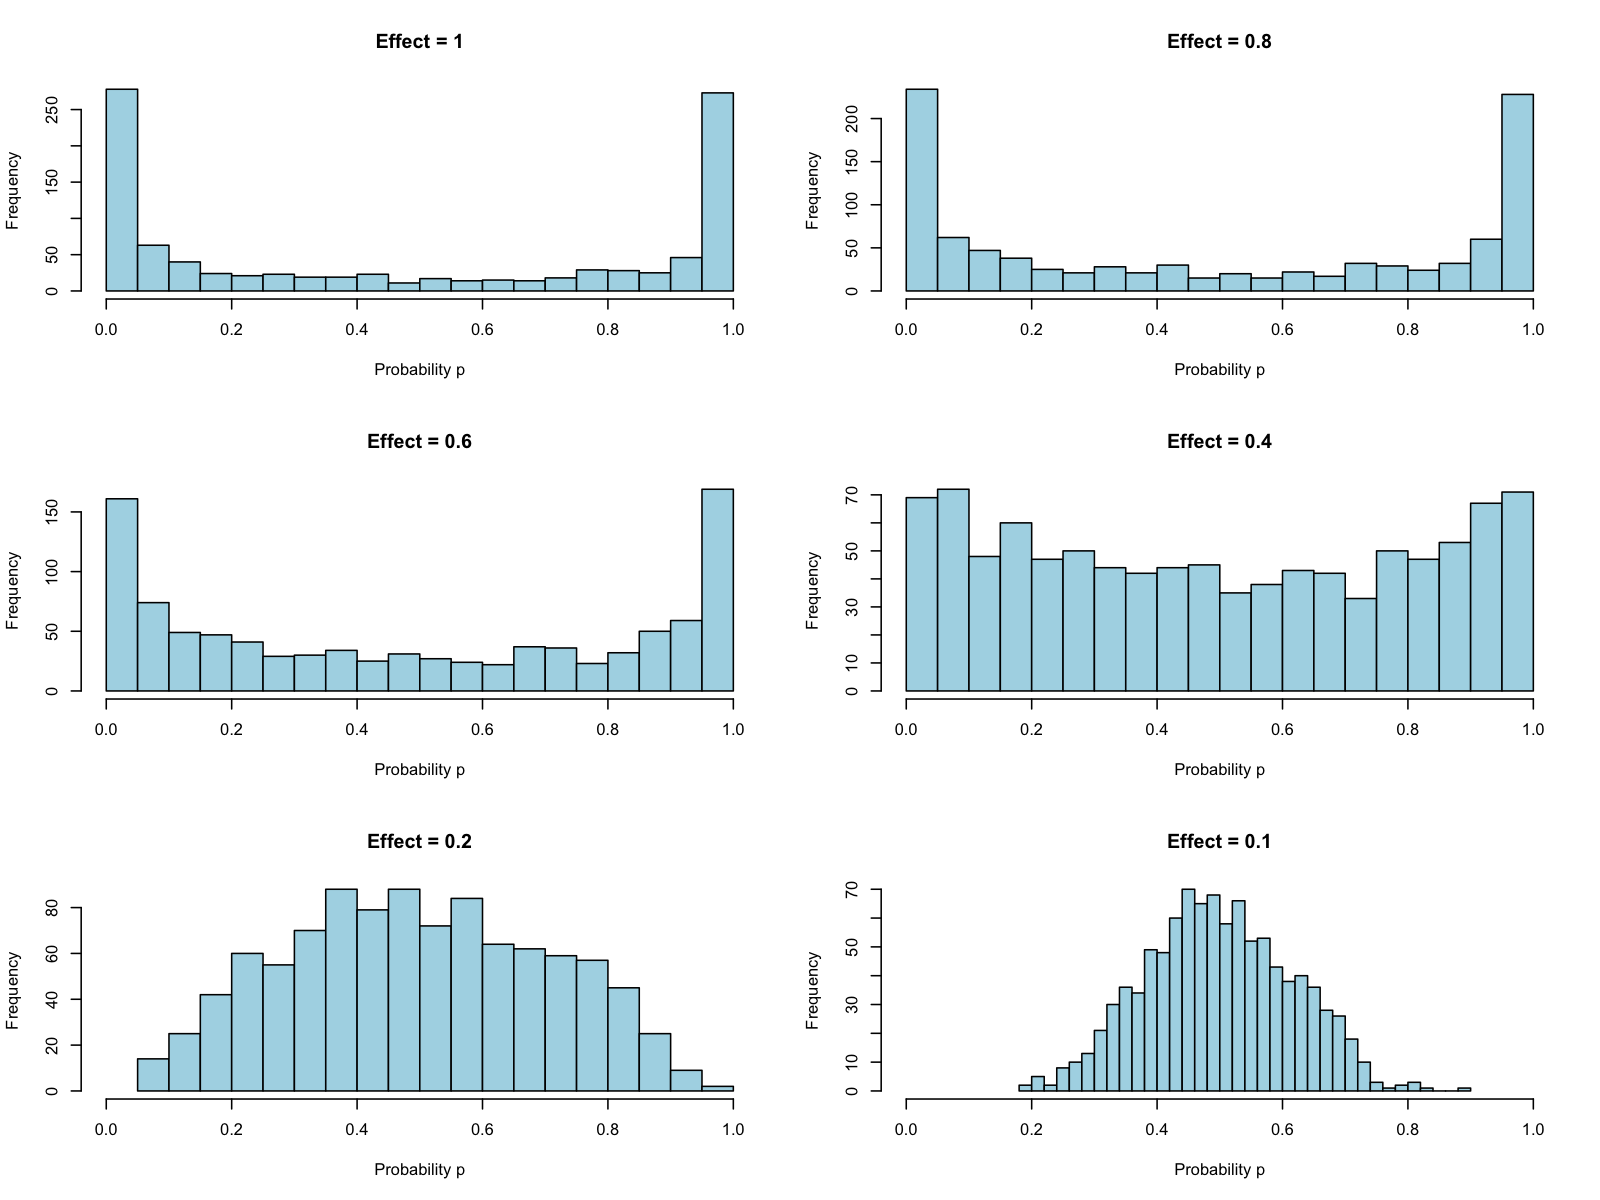
\includegraphics[width=0.8\textwidth]{sim2_p_dist.png} 
  \caption{Distribution of success probability \( p \) at different \( b \) values in Simulation 2.}
	\label{fig:sim2_p_dist} 
\end{figure}

\FloatBarrier

\subsection*{Group Mean Difference}

Using the selected values of \( \beta \) and \( b \), figure \ref{fig:group_diff1} and \ref{fig:group_diff2} depict the group mean difference in covariate values between instances where \( y = 1 \) and \( y = 0 \) in both the pixel space and frequency space for Simulation 1 and 2, respectively. For Simulation 1, as shown in Figure \ref{fig:group_diff1}, the heatmap in the pixel space reveals that the central region with non-zero coefficients in \( \beta \) corresponds to higher mean covariate values, which is consistent with the heatmap of \( \beta \) in Figure \( \ref{fig:coefs_sim1} \). Similarly, regions with higher or lower values in the frequency space match the corresponding values in the coefficients. A similar pattern is observed in Simulation 2, as illustrated in Figures \ref{fig:group_diff2} and \ref{fig:coefs_sim2}, where the heatmaps for both the pixel and frequency spaces demonstrate alignment between covariate values and the corresponding non-zero coefficients. 

\begin{figure}[h!] 
	\centering
	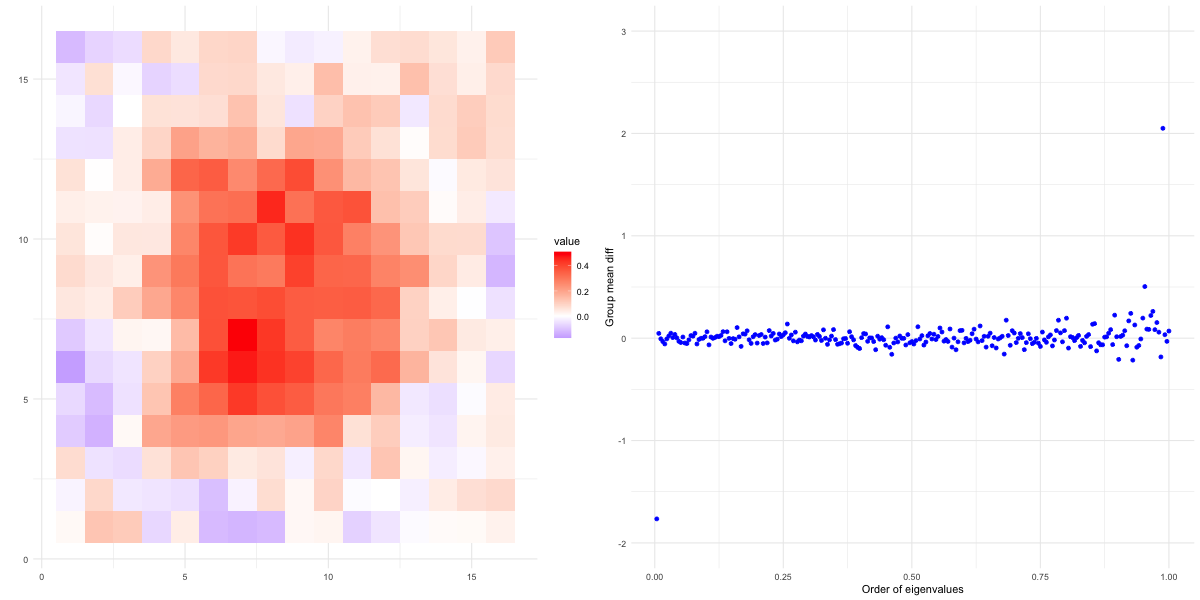
\includegraphics[width=0.9\textwidth]{group_mean_diff_sim1.png}
	\caption{Group mean difference in covariate values between instances where \( y = 1 \) and \( y = 0 \) in Simulation
  1, shown for both the pixel space (left) and frequency space (right).}
	\label{fig:group_diff1}
\end{figure}

\begin{figure}[h!] 
	\centering
	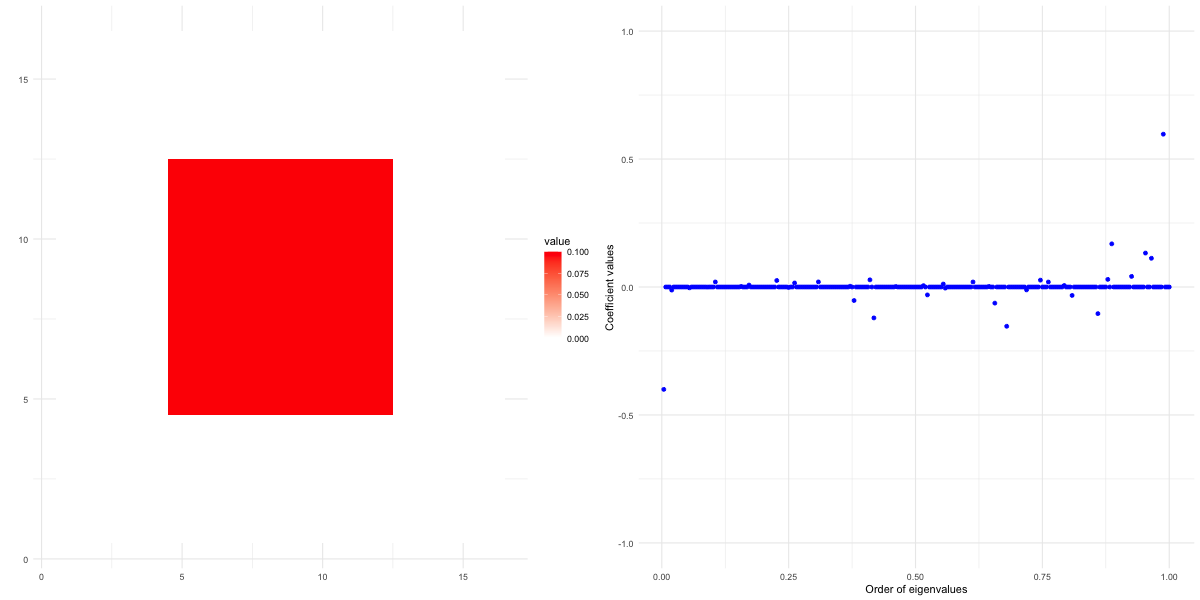
\includegraphics[width=0.9\textwidth]{actual_coefs_sim1.png}
  \caption{Actual coefficients in Simulation 1 for the pixel space (left) and frequency space (right).}
  \label{fig:coefs_sim1}
\end{figure}

\begin{figure}[h!] 
	\centering
	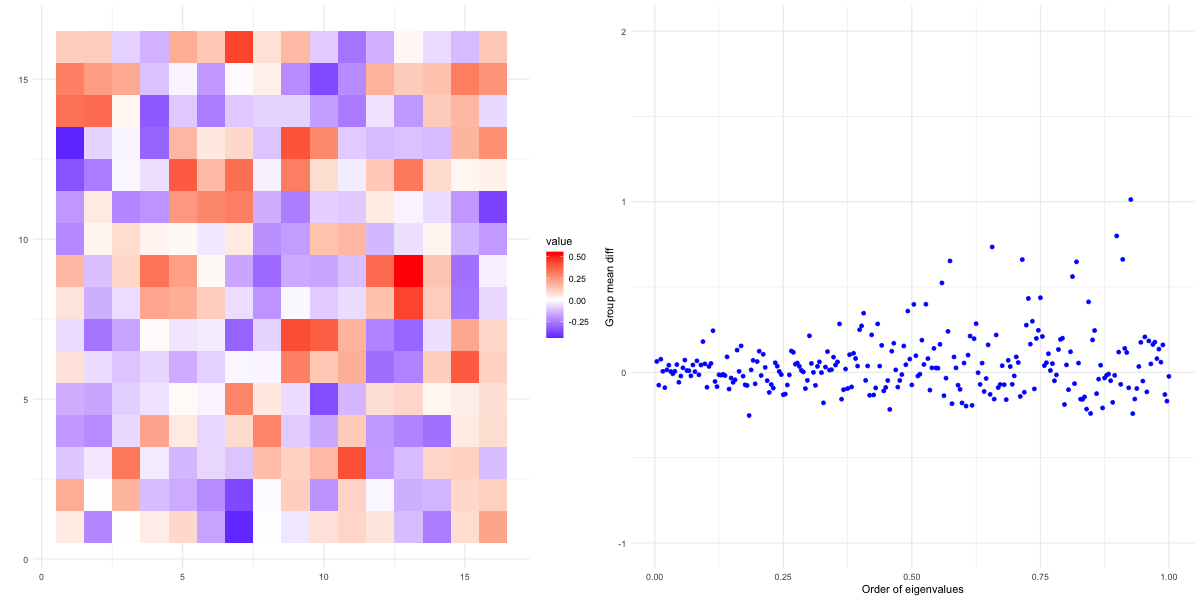
\includegraphics[width=0.9\textwidth]{group_mean_diff_sim2.png}
	\caption{Group mean difference in covariate values between instances where \( y = 1 \) and \( y = 0 \) in Simulation 2.}
	\label{fig:group_diff2}
\end{figure}

\begin{figure}[h!] 
	\centering
	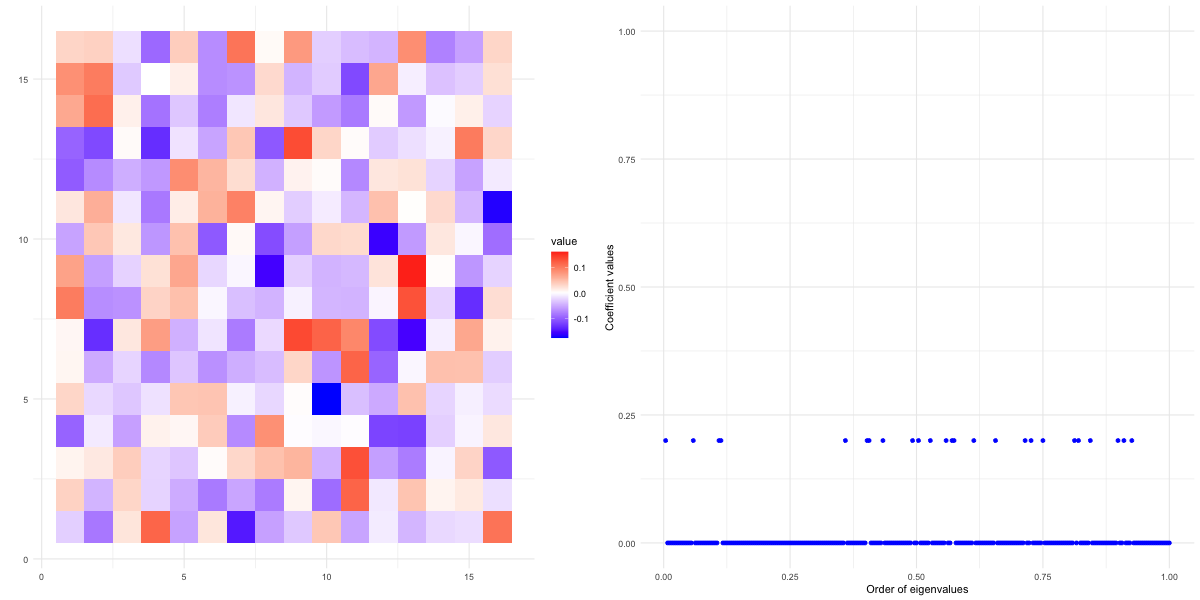
\includegraphics[width=0.9\textwidth]{actual_coefs_sim2.png}
  \caption{Actual coefficients in Simulation 2 for the pixel space (left) and frequency space (right).}
  \label{fig:coefs_sim2}
\end{figure}

\FloatBarrier

\subsection*{Model Performance Evaluation: AUC and Accuracy}

To assess the performance of models fitted with covariates from the pixel space versus the frequency space, we evaluated
the area under the curve (AUC) and prediction accuracy. LASSO models were trained using cross-validation by splitting
each set of 1000 simulated observations into 80\% training and 20\% test sets. This process was repeated 500 times.
Table~\ref*{tab:auc_acc_table} presents the average AUCs and accuracies over the 500 iterations. Regardless of whether
sparsity is assumed in the pixel space (Simulation 1) or the frequency space (Simulation 2), models fitted in the
frequency space consistently outperformed those fitted in the pixel space. Specifically, in Simulation 1, using
`lambda.min` as the regularization value, models fitted with covariates from the pixel space achieved an AUC of
0.803 (SE = 0.031) and an accuracy of 72.6\% (SE = 0.032). In contrast, models fitted with covariates from the 
frequency space achieved a slightly higher AUC of 0.826 (SE = 0.028) and a higher accuracy of
74.5\% (SE = 0.030). A similar trend was observed in Simulation 2, with models fitted in the frequency space
demonstrating superior performance regardless of the regularization parameter used.

\begin{table}[h!]
\centering
\caption{Comparison of AUC and accuracy between models fitted in the pixel space and frequency space across 500 iterations for Simulation 1 and Simulation 2.}
\label{tab:auc_acc_table}
\begin{tabular}{l|cc|cc}
\toprule
\textbf{Simulation} & \multicolumn{2}{c}{\textbf{Model in Pixel Space}} & \multicolumn{2}{c}{\textbf{Model in Frequency Space}} \\ 
\midrule
& \textbf{AUC (SE)} & \textbf{Accuracy (SE)} & \textbf{AUC (SE)} & \textbf{Accuracy (SE)} \\ 
\midrule
\textbf{Simulation 1} & & & & \\
lambda.min & 0.803 (0.031) & 0.726 (0.032) & 0.826 (0.028) & 0.745 (0.030) \\
lambda.1se & 0.800 (0.032) & 0.722 (0.032) & 0.826 (0.029) & 0.745 (0.031) \\ 
\midrule
\textbf{Simulation 2} & & & & \\
lambda.min & 0.755 (0.036) & 0.684 (0.034) & 0.812 (0.030) & 0.732 (0.032)  \\
lambda.1se & 0.735 (0.039) & 0.669 (0.038) & 0.812 (0.031) & 0.732 (0.032) \\
\bottomrule
\end{tabular}
\end{table}

\subsection*{Coefficients Estimation}

The mean estimated coefficients in both the pixel space and frequency space were calculated for Simulation 1 and Simulation 2. Figure \ref{fig:beta_estimates} displays the mean estimated \( \beta \) values. The left column shows the estimates when models were fitted using \texttt{lambda.min}, while the right column corresponds to models fitted using \texttt{lambda.1se}. The top row presents the results for Simulation 1, and the bottom row for Simulation 2. When comparing these estimated \( \beta \) values to the actual coefficients shown in Figures \ref{fig:coefs_sim1} and \ref{fig:coefs_sim2}, it is evident that the estimated values closely align with the true coefficients.

Figure \ref{fig:b_estimates} presents the mean estimated \( b \) values plotted against the ordered eigenvalues. The eigenvalues are ranked from smallest to largest, with the smallest assigned an order of 1. To standardize the scale, the orders are then divided by the total number of eigenvalues, resulting in values between 0 and 1 on the x-axis. In Simulation 1, the number of non-zero coefficient estimates closely matches the true \( b \) values shown in Figure \ref{fig:coefs_sim1}. These non-zero coefficients are primarily concentrated among the largest eigenvalues, indicating that the model correctly identifies the most significant components. In contrast, Simulation 2 shows that non-zero coefficient estimates are more uniformly distributed along the x-axis.

\begin{figure}[h!] 
	\centering
  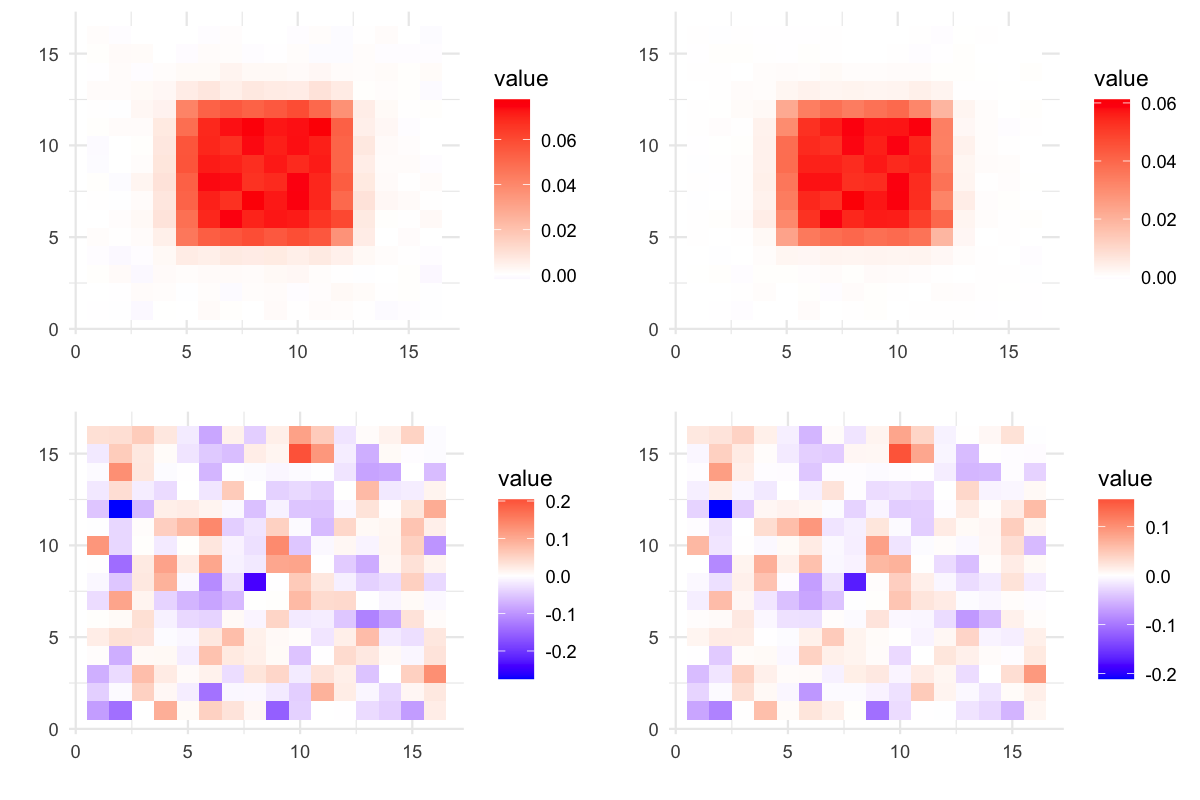
\includegraphics[width=0.9\textwidth]{beta_estimates.png} 
  \caption{Mean estimated \( \beta \) values across simulations, with models fitted using \texttt{lambda.min} (left) and
  \texttt{lambda.1se} (right). The top row shows results for Simulation 1, while the bottom row shows results for Simulation 2.}
	\label{fig:beta_estimates} 
\end{figure}

\begin{figure}[h!] 
	\centering
  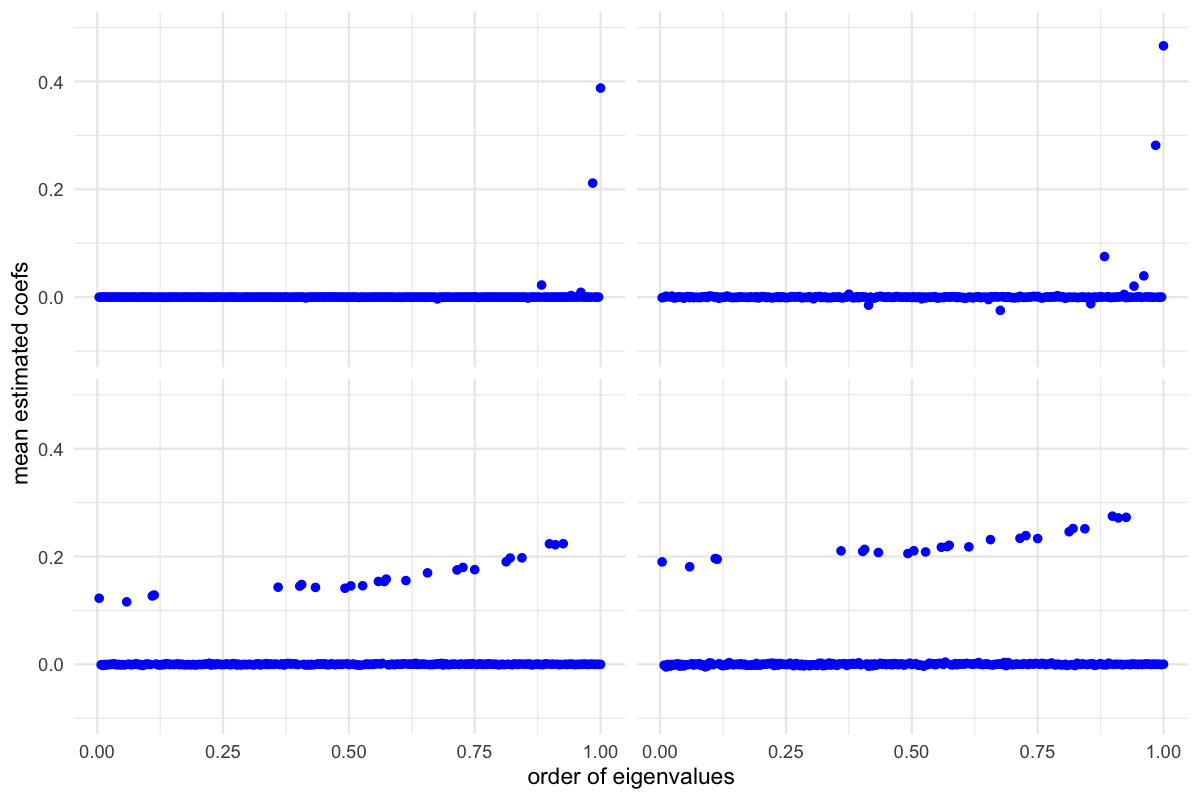
\includegraphics[width=0.9\textwidth]{b_estimates.png} 
  \caption{Mean estimated \( b \) values across simulations, plotted against ordered eigenvalues. Models fitted using
  \texttt{lambda.min} are on the left and models fitted with \texttt{lambda.1se} on the right. The top row shows results for Simulation 1, while the bottom row shows results for Simulation 2.}
  \label{fig:b_estimates} 
\end{figure}

\FloatBarrier

\subsection*{Significant P-values}

\begin{figure}[h!] 
	\centering
  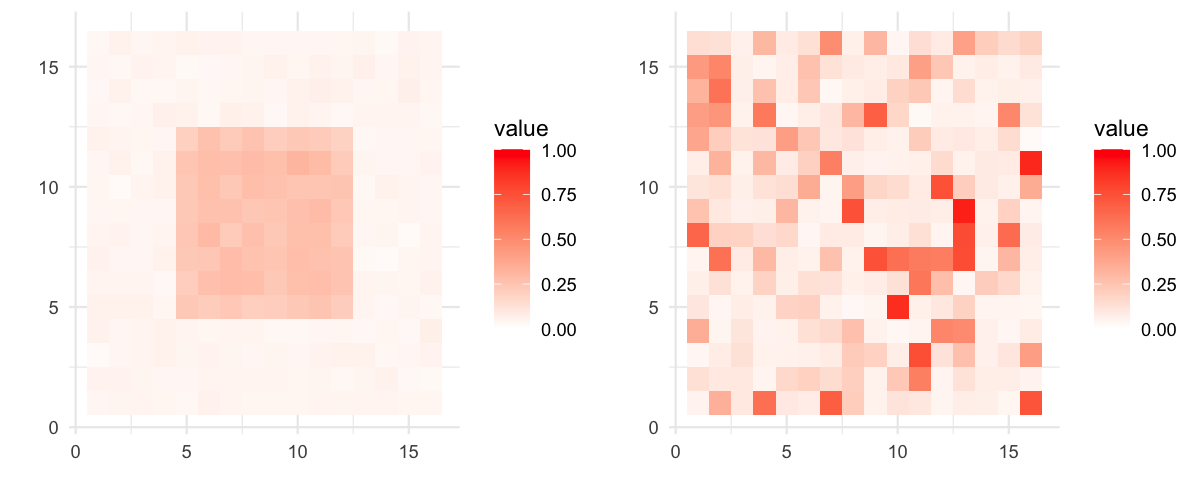
\includegraphics[width=0.9\textwidth]{perc_sign_pvals_hdi_beta.png} 
  \caption{Percentage of significant p-values for elements of \( \beta \) when fitting models in the pixel space in
  Simulation 1 (left) and Simulation 2 (right).}
	\label{fig:perc_sign_beta} 
\end{figure}

\begin{figure}[h!] 
	\centering
  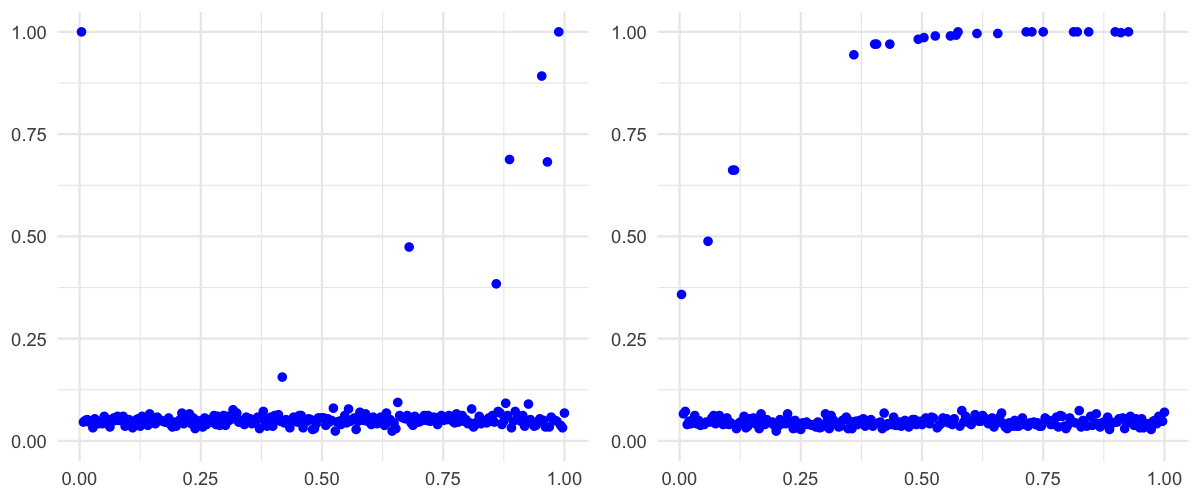
\includegraphics[width=0.9\textwidth]{perc_sign_pvals_hdi_b.png} 
  \caption{Percentage of significant p-values for elements of \( b \) across ordered eigenvalues in both simulations.}
	\label{fig:perc_sign_b} 
\end{figure}

\FloatBarrier

Figure~\ref*{fig:top_bottom_eigvecs} presents the frequencies associated with the top three eigenvalues, which represent the dominant patterns in the pixel space. The frequency associated with the smallest eigenvalue is also shown, highlighting the least significant variance.

\begin{figure}[h!] 
	\centering
	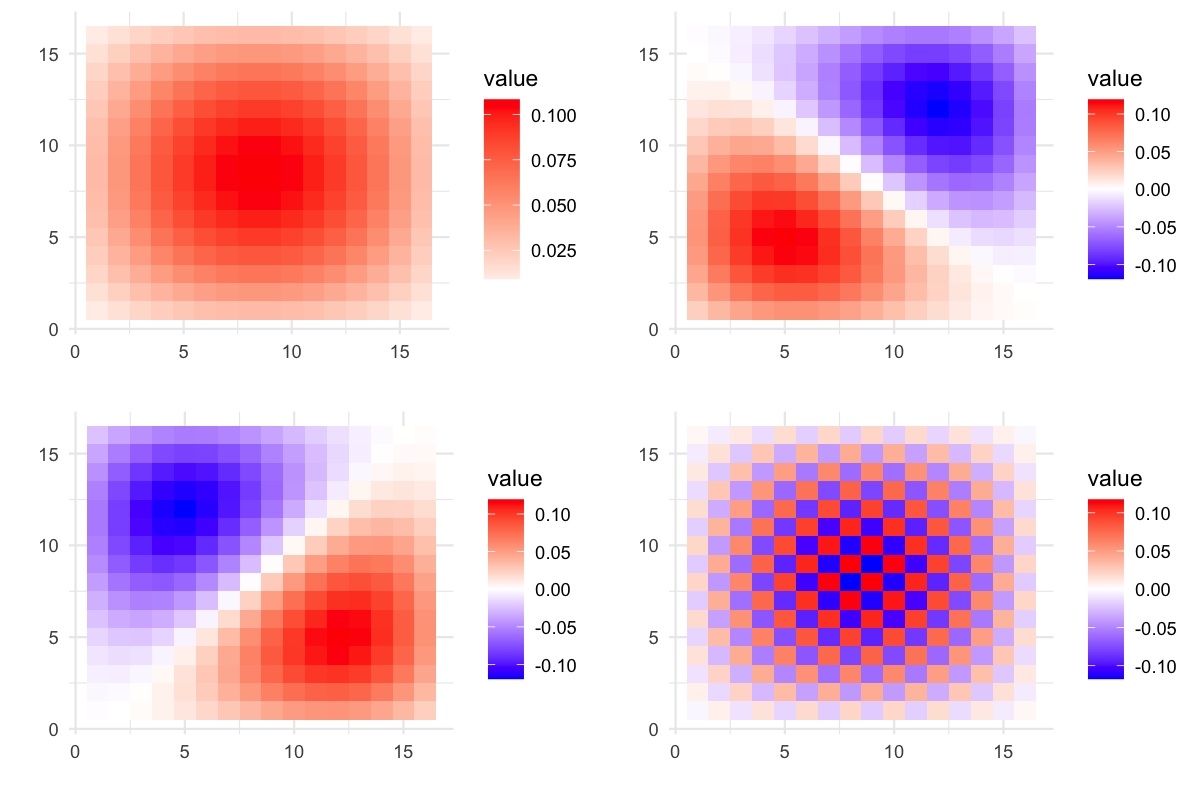
\includegraphics[width=0.8\textwidth]{top_bottom_eigvecs.png} 
\caption{Frequencies associated with the top three eigenvalues (top row and bottom left) and the frequency associated with the smallest eigenvalue (bottom right), highlighting the primary and least significant patterns in the pixel space.}
	\label{fig:top_bottom_eigvecs} 
\end{figure}


\end{document}
